\documentclass[border=6pt]{standalone}
\usepackage{tikz}
\usetikzlibrary{arrows.meta,positioning}
\begin{document}
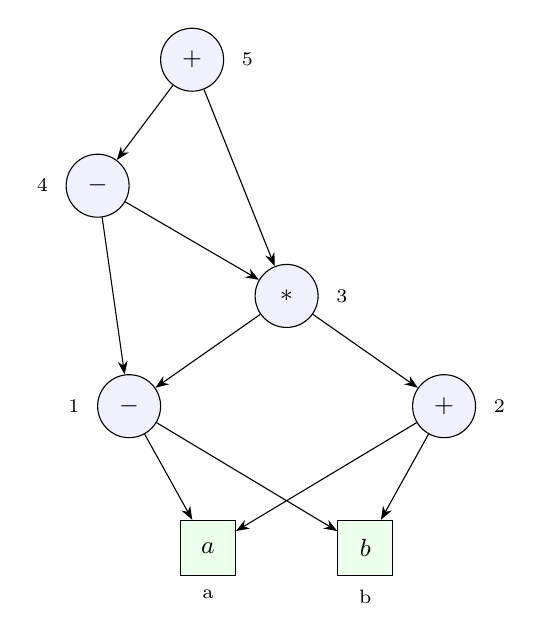
\begin{tikzpicture}[>=Stealth,font=\small,
 op/.style={draw,circle,minimum size=0.8cm,inner sep=0pt,fill=blue!6},
 lf/.style={draw,rectangle,minimum size=0.7cm,inner sep=0pt,fill=green!8}]
\node[op] (n5) at (1.2,5.6) {$+$}; \node[right=0.1cm of n5,font=\scriptsize] {5};
\node[op] (n4) at (0,4) {$-$}; \node[left=0.1cm of n4,font=\scriptsize] {4};
\node[op] (n3) at (2.4,2.6) {$*$}; \node[right=0.1cm of n3,font=\scriptsize] {3};
\node[op] (n1) at (0.4,1.2) {$-$}; \node[left=0.1cm of n1,font=\scriptsize] {1};
\node[op] (n2) at (4.4,1.2) {$+$}; \node[right=0.1cm of n2,font=\scriptsize] {2};
\node[lf] (a) at (1.4,-0.6) {$a$}; \node[below=0.05cm of a,font=\scriptsize] {a};
\node[lf] (b) at (3.4,-0.6) {$b$}; \node[below=0.05cm of b,font=\scriptsize] {b};
\draw[->] (n5) -- (n4);
\draw[->] (n5) -- (n3);
\draw[->] (n4) -- (n1);
\draw[->] (n4) -- (n3);
\draw[->] (n3) -- (n1);
\draw[->] (n3) -- (n2);
\draw[->] (n1) -- (a);
\draw[->] (n1) -- (b);
\draw[->] (n2) -- (a);
\draw[->] (n2) -- (b);
\end{tikzpicture}
\end{document}
